\documentclass[a4paper, 10pt]{article}

%\usepackage{scalefnt}
%\usepackage{parcolumns}

\usepackage{newclude}
% Zum Einbinden in die Zusammenfassungs-files

\usepackage{amsmath,amsthm,amsfonts,amssymb} % Verbesserter Mathesatz
\usepackage{algorithm2e}
\usepackage{bigfoot} % komplexe Fußnotenapparate(Fußnoten in Fußnoten und andere Späße)%
\usepackage{colortbl}
\usepackage[T1]{fontenc} % normaler erweitere Zeichnesatz
\usepackage{framed, color}  % Ramenpaket für zum Einfügen von schönen Ramen
\usepackage{graphicx}
\usepackage{hyperref} %used for link to creative commons license
\usepackage{listings} %for code-listings (inkl. Tab-Styling)
\usepackage{marvosym}
\usepackage{marginnote}
\usepackage{microtype} % div. Verbesserungen des Schriftsatzes (Grauwert, opt. Randausgleich, Zeilenumbruch)
%\usepackage{multirow}
\usepackage{multicol} %use this with next line for vertical divided environment
%\setlength\columnseprule{.4pt}:465
\usepackage[ngerman]{babel} % Neue Rechtschreibung
\usepackage{pifont}
\usepackage[sans]{dsfont} %für alternative Mengensymbole
\usepackage{stmaryrd} %u.a. für \lightning
\usepackage{tikz} % für Diagramme(Dia!) und Bilder (z.B. *.eps)/für ER-Diagramme/für UML-Diagramme
%\usepackage{tikz-er2} %  er-diagramme
\usepackage{tikz-uml} % uml-Diagramme
\usepackage{units} % z.B. fuer \nicefrac{}{}
\usepackage[utf8]{inputenc} % utf8 für den Editor
\usepackage{wasysym} %u.a. für \lightning
\usepackage{xcolor}


\usetikzlibrary{shapes,decorations,arrows,fit,backgrounds} %Zum diversen zeichen%
%\usetikzlibrary{automata} % für den CFlipper, wenn es den soweit ist			%
\usetikzlibrary{positioning} % positionierung
%\usetikzlibrary{shadows} % fuer schoene schlagschatten
\usetikzlibrary{automata} % für Automaten

%%%%%%%%%%%%%%%%%%%%%%%%%%%
%  Formatierung der Seite
%%%%%%%%%%%%%%%%%%%%%%%%%%%
\usepackage{fancyhdr}
\pagestyle{fancy}		% für den footer										%
\renewcommand{\headrulewidth}{0pt} % damit oben kein dummer Strich kommt		%
\fancyhead{}
\topmargin -2cm 		% Oberer Rand											%
\textheight 25cm		% Texthöhe												%
\textwidth 16.0 cm		% Textbreite											%
\oddsidemargin -0.1cm 	% Warum?												%
\newcommand{\Gruppe}[2]
{
	\lfoot{#1}
	\rfoot{#2}
}
\colorlet{shadecolor}{gray!25} % Farbe für graue Box definieren
%%%%%%%%%%%%%%%%%%%%%%%%%%%%%%%%%%%%%%%%%%%%%%%%%%%%%%%%%%%%%%%%%%%%%%%%%%%%%%%%%
%Farben die definiert werden zum schreiben und zeichnen							%
%%%%%%%%%%%%%%%%%%%%%%%%%%%%%%%%%%%%%%%%%%%%%%%%%%%%%%%%%%%%%%%%%%%%%%%%%%%%%%%%%
\xdefinecolor{schwarz}{HTML}{000000}
\xdefinecolor{dunkelGruen}{HTML}{007D00}
\xdefinecolor{dunkelBlau}{HTML}{0000A0}
\xdefinecolor{dunkelRot}{HTML}{A00000}
\xdefinecolor{dunkelGelb}{HTML}{FFAA00}
\xdefinecolor{hellesGelb}{HTML}{FFCC00}
\colorlet{dGreen}{dunkelGruen}
\colorlet{dBlue}{dunkelBlau}
\colorlet{dRed}{dunkelRot}
\colorlet{dYellow}{dunkelGelb}

%%%%%%%%%%%%%%%%%%%%%%%%%%%%%%%%%%%%%%%%%%%%%%%%%%
%Farbliche Ausgaben:
%Parameter #1: Text oder Mathematische formel...
%z.B. : \gruen{Hallo Welt Test!}
%%%%%%%%%%%%%%%%%%%%%%%%%%%%%%%%%%%%%%%%%%%%%%%%%%

\newcommand{\yellow}[1]{\textcolor{dYellow}{#1}}
\newcommand{\gray}[1]{\textcolor{gray}{#1}}
\newcommand{\red}[1]{\textcolor{red}{#1}}
\newcommand{\green}[1]{\textcolor{green}{#1}}
\newcommand{\blue}[1]{\textcolor{blue}{#1}}
\newcommand{\dGreen}[1]{\textcolor{dGreen}{#1}}
\newcommand{\dBlue}[1]{\textcolor{dBlue}{#1}}
\newcommand{\dRed}[1]{\textcolor{dRed}{#1}}

%%%%%%%%%%%%%%%%%%%%%%%%%%%%%%%%%%%%%%%%%%%%%%%%
%Konfiguration für das darstellen von Quelltext
%%%%%%%%%%%%%%%%%%%%%%%%%%%%%%%%%%%%%%%%%%%%%%%%
\lstset
{
	language=Java, % oder C++, Pascal, {[77]Fortran}, ...
	numbers=left, % Position der Zeilennummerierung
	firstnumber=auto, % Erste Zeilennummer
	basicstyle=\ttfamily, % Textgröße des Standardtexts
	keywordstyle=\ttfamily\color{dRot}, % Formattierung Schlüsselwörter
	commentstyle=\ttfamily\color{dGruen}, % Formattierung Kommentar
	stringstyle=\ttfamily\color{dBlau}, % Formattierung Strings
	numberstyle=\tiny, % Textgröße der Zeilennummern
	stepnumber=1, % Angezeigte Zeilennummern
	numbersep=5pt, % Abstand zw. Zeilennummern und Code
	aboveskip=15pt, % Abstand oberhalb des Codes
	belowskip=11pt, % Abstand unterhalb des Codes
	captionpos=b, % Position der Überschrift
	xleftmargin=10pt, % Linke Einrückung
	frame=single, % Rahmentyp
	breaklines=true, % Umbruch langer Zeilen
	showstringspaces=false, % Spezielles Zeichen für Leerzeichen
	tabsize=2,
	texcl=true
}

%%%%%%%%
% Kopf
%%%%%%%%
\newcommand{\Header}[3]
{
	{\footnotesize \parindent0em
		{\sc Universität Konstanz}                \hfill #1 \\
		{\sc Fachbereich Informatik \& Informationswissenschaft} \hfill #2 \\
		#3 \hfill \today
	}
}

%%%%%%%%%%%%%%%%%%%%%%%
% load some java code
% \loadJava{file}
%%%%%%%%%%%%%%%%%%%%%%%
\newcommand{\loadJava}[1]
{
	\lstinputlisting[language=Java]{#1.java}
}

%%%%%%%%%%%%%%%%%%%%%%%
% load some cpp code
% \loadCpp{file.cpp}
%%%%%%%%%%%%%%%%%%%%%%%
\newcommand{\loadCpp}[1]
{
	\lstinputlisting[language=C++]{#1}
}

%%%%%%%%%%%%%%%%%%%%%%%%%%%%%
% load some code
% \loadCode{Python}{file.py}
%%%%%%%%%%%%%%%%%%%%%%%%%%%%%
\newcommand{\loadCode}[2]
{
	\lstinputlisting[language=#1]{#2}
}

%%%%%%%%%%%%%%%%%%%%%%%%%%%%%%%%%%%%%%%%%%%%%%%%%%%%%%%%%%%%%%%%%%%%%%%
% some symbols
%%%%%%%%%%%%%%%%%%%%%%%%%%%%%%%%%%%%%%%%%%%%%%%%%%%%%%%%%%%%%%%%%%%%%%%
\newcommand{\correct}{\green{\text{\ding{52}}}} %for use in text and math
\newcommand{\wrong}{\red{\text{\ding{56}}}} %for use in text
\newcommand{\tflash}{$\yellow{\lightning}$} %for use in text
\newcommand{\mflash}{\yellow{\lightning}} %for use in math
\newcommand{\follows}{$\Rightarrow$} %used so often...
\newcommand{\good}{\item[\dGreen{\ding{58}}]} %an item with a green plus as bullet point
\newcommand{\bad}{\item[\red{\Emailct}]} %better icon for bad items
\newcommand{\note}[1]{\red{\marginnote{#1}}} %add a red margin note
\newcommand{\fitem}{\item[\follows]} %items with a follows arrow
\newcommand{\hm}{\ensuremath{\overset{-\mkern-11mu-\mkern-3.5mu\rhook}{\smash{\odot}\rule{0ex}{.46ex}}\underline{\hspace{0.5em}}\overset{-\mkern-11mu-\mkern-3.5mu\rhook}{\smash{\odot}\rule{0ex}{.46ex}}}}

%%%%%% make emph bold instead of italic %%%%%
\makeatletter
\DeclareRobustCommand{\em}{%
  \@nomath\em \if b\expandafter\@car\f@series\@nil
  \normalfont \else \bfseries \fi}
\makeatother

%%%%%%%%%%%%%%%%%%%%%%%%%%%%%%%%%%%%%%
% languages for \loadCode
%ABAP		IDL				Plasm
%ACSL		inform			POV
%Ada		Java			Prolog
%Algol		JVMIS			Promela
%Ant		ksh				Python
%Assembler	Lisp			R
%Awk		Logo			Reduce
%bash		make			Rexx
%Basic		Mathematica1	RSL
%C			Matlab			Ruby
%C++		Mercury			S
%Caml		MetaPost		SAS
%Clean		Miranda			Scilab
%Cobol		Mizar			sh
%Comal		ML				SHELXL
%csh		Modula-2		Simula
%Delphi		MuPAD			SQL
%Eiffel		NASTRAN			tcl
%Elan		Oberon-2		TeX
%erlang		OCL				VBScript
%Euphoria	Octave			Verilog
%Fortran	Oz				VHDL
%GCL		Pascal			VRML
%Gnuplot	Perl			XML
%Haskell	PHP				XSLT
%HTML		PL/I
%%%%%%%%%%%%%%%%%%%%%%%%%%%%%%%%%%%%%%

\begin{document}

\Gruppe{Stephan Heidinger}{fses 08}
\Header{Functional Safety in Embedded Systems}{Session 08 - Critical System Development}

%\begin{shaded}
%Dieses Dokument wurde unter der Creative Commons - Namensnennung-NichtKommerziell-Weitergabe unter gleichen Bedingungen (\textbf{CC by-nc-sa}) veröffentlicht. Die Bedingungen finden sich unter \href{http://creativecommons.org/licenses/by-nc-sa/3.0/de}{diesem Link}. \\
%\centerline{
\includegraphics[scale=1]{../cc-by-nc-sa.png} }
%\end{shaded}

%\textit{\ensuremath{\overset{-\mkern-11mu-\mkern-3.5mu\rhook}{\smash{\odot}\rule{0ex}{.46ex}}\underline{\hspace{0.5em}}\overset{-\mkern-11mu-\mkern-3.5mu\rhook}{\smash{\odot}\rule{0ex}{.46ex}}}
%Find any errors? Please send them back, I want to keep them!}

%\section*{something}

%\section*{more}

\section*{development of safety-critical applications}
\begin{itemize}
    \item only fault tolerance depends on technical solution, the others depend on development process
    \item development process helps improve efficiency, efficacy and is needed for certification
    \item Higher level of criticality \follows more formality
    \item domain specific standards/ processes
\end{itemize}

\subsection*{What makes a system complex?}
essential complexity (Dvorak (2009))
\begin{enumerate}
    \item \emph{Functions to be performed:} wide range of different functions, tasks regulated by complex physical or control laws, implement complex control logic
    \item \emph{Operating Environment:} harsh environment, tight timing constraints, input from different sensors, output to different actuators
    \item \emph{Criticality:} fail-operational, implement safety functions \follows more complex logic
\end{enumerate}

\subsection*{What makes the development complex?}
\subsubsection*{Novelty}
\begin{itemize}
    \item technology used for the first time ever (at least in domain)
    \item first use of technology in company
\end{itemize}

\subsubsection*{Schedule Constraints}
\begin{itemize}
    \item Critical Path: sequence of events with least lax, any delay in critical path will increase time to completion
    \item nearly critical paths \follows short delay ok, more delay not ok
    \item with tight timing/ staffing \follows number of nearly critical paths increase
    \item intentionally add slack time between events (during planing) s.t. delay not that bad
\end{itemize}

\subsubsection*{Team}
\begin{itemize}
    \item people are stupid
\end{itemize}

\subsubsection*{Geographical Distribution}
\begin{itemize}
    \item can be good or not good
    \good mitigate staffing constraints
    \good hire people not available locally
    \good work around the clock
    \bad information flow can degrade
    \bad different laws in different countries, example: A380
\end{itemize}

\subsubsection*{Organizations Maturity}
\begin{itemize}
    \item \emph{Capability Maturity Model Integration} (CMMI), framework to measure and improve organizations maturity
    \begin{itemize}
        \item initial to optimized
    \end{itemize}
    \item standardized production practices
\end{itemize}

\subsubsection*{Tools}
\begin{itemize}
    \item tools support information intensive activities
    \item e.g. wind tunnel simulation directly from CAD
\end{itemize}

\subsection*{Measuring the Impact of Complexity}
\begin{itemize}
    \item COCOMO and Function Point (FP) well known to estimate effort required to develop system
    \item COCOMO
    \begin{itemize}
        \item $Effort=A\cdot (SIZE)^{B+SF}\cdot EAF$
        \begin{description}
            \item[$Effort$] effort needed to develop a system
            \item[$SIZE$] predicted size of system in LOC
            \item[$A, B$] company-wide constants
            \item[$SF$] the \emph{Scale Factor}: project dependent, models economy, diseconomy, exponential
            \item[$EAF$] the \emph{Effort Adjustment Factor}: project dependent, multiplicative
        \end{description}
        \item parameters measuring the capability of the performing organization
        \begin{description}
            \item[Precedentness] experience of company with system
            \item[Flexibility] constraints related to project execution, schedule constraints
            \item[Team] team maturity, experience, cohesion
            \item[Risk Resolution] how are risks managed
            \item[Process Maturity] organization maturity according to CMMI model
        \end{description}
        \item adjustment factors $EAF$ more complex
        \begin{itemize}
            \item Early Design Model (after requirements)
            \item Post-Architecture Model (after architecture definition)
            \item 4 classes
            \begin{description}
                \item[Product] measure complexity of system, required reliability, database size, product complexity, required usability
                \item[Platform] measure aspects related to platform, in which system will run, execution time constraints, main storage constraints, platform volatility
                \item[Personnel] measure the capability of personnel in project, general experience, specific experience (platform, language, tool), staff turnover
                \item[Project] measure project related characteristics, communication, team geographical distribution
            \end{description}
        \end{itemize}
    \end{itemize}
\end{itemize}

\subsection*{From System to Process}
\begin{itemize}
    \item Top-down decomposition is effective approach to manage complexity
    \item can be represented as a tree
    \item different approaches to define and organize trees
    \begin{itemize}
        \item function trees: decomposition according to function
        \item product trees: decomposition according to components
        \item mixed models
    \end{itemize}
    \item work breakdown structures (WBS): hierarchies enriched with some stuff to know what to do
\end{itemize}

\subsubsection*{Obligations and Benefits}
\begin{itemize}
    \item term from ``design by contract''
    \item effective for allocation of functional and safety requirements
    \item advantages:
    \begin{itemize}
        \good During Design: top-down fashion, validate decomposition and architectural choices
        \good During Verification: bottom-up: demonstrate, that each element correctly implements the safety requirements allocated
    \end{itemize}
\end{itemize}

\subsubsection*{Early Assessment}
\begin{itemize}
    \item initial assessment of system, which architecture, which requirement on which component
    \item fault injection often by hand
    \item theorem proving
    \begin{description}
        \item[increasing] (TI) abstraction \follows results in concrete space also hold in abstract space
        \item[constant] (TC) abstraction \follows results in abstract space hold iff the hold in the concrete space
        \item[decreasing] (TD) abstraction \follows results in the abstract space hold in the concrete space
    \end{description}
    \item abstractions used as a heuristic for simplifying the proof of theorems \follows divide and conquer

\end{itemize}

\subsection*{a general development framework}
\begin{itemize}
    \item time flows from right to left \follows different stages, that characterize development of system
    \item by row: activities in a workflow
    \item by column: development progress
    \begin{center}
        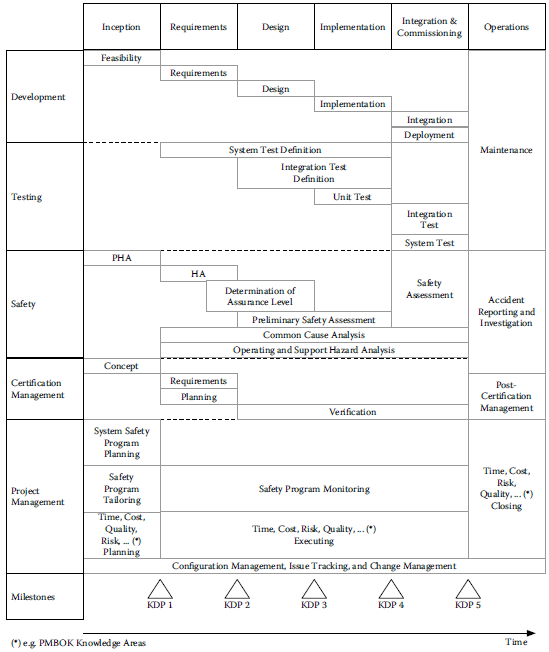
\includegraphics[width=\linewidth]{images/genDev.png}
    \end{center}
\end{itemize}

\subsubsection*{Phases and Phase Transition}
\begin{itemize}
    \item transition from concept to product through phases
    \begin{description}
        \item[Inception] need/ opportunity for new system/ revising system is drafted, elaborated, evaluated \\ feasibility risks, forecast profit\dots
        \item[Requirements] characteristics of system are defined, analysis of environment
        \item[Design] structure and design are drafted and evaluated, safety-critical components are individuated, design alternatives are evaluated, choices for critical and non-critical components, activities for certification
        \item[Implementation] development of system according to design phase, development and testing can be in parallel, unit testing
        \item[Integration and Commissioning] components are integrated into final assembly, certification takes place, system is put into operation
        \item[Operations] system is maintained to ensure service
    \end{description}
    \item transitions are determined by milestones
    \item results of verification are used with complementary goals:
    \begin{enumerate}
        \item formal verification point to decide \emph{transition to next phase}
        \item formal verification to \emph{decide whether to continue project}
    \end{enumerate}
\end{itemize}


\subsubsection*{Comparison with Other Frameworks}
\begin{description}
    \item[Rational Unified Process] (RUP)
    \begin{itemize}
        \item organize development into four phases: \emph{Inception, Elaboration, Construction, Transition}
        \begin{itemize}
            \item four milestones define phase transitions
            \begin{description}
                \item[Life-Cycle Objectives] concludes Inception phase, provides stakeholders with information necessary to decide, if project is to be continued
                \item[Life-Cycle Architecture] concludes elaboration phase, provides stable version of vision, requirements, architecture, prototype
                \item[Initial Operational Capability] concludes Construction phase, system ready to deploy, all other stuff (e.g. training) in place
                \item[Product Release] concludes Transition, verify that the system has initial goals and met stakeholders expectation
            \end{description}
        \end{itemize}
    \end{itemize}
    \item[European Space Agency] (ESA)
    \begin{itemize}
        \item seven phases
        \begin{description}
            \item[Phase 0, Mission analysis and needs identification] goals, preliminary studies for market opportunity, cost, main risk
            \item[Phase A, Feasibility] main project plan outline, technical feasibility, Phase 0 gets refined
            \item[Phase B, Preliminary Definition] previous phases refined, technical solutions committed to, pre-development on most critical technologies, safety assessment
            \item[Phase C, Detailed Information] system is developed, detailed designs, engineering models, critical components
            \item[Phase D, Qualification and Production] system is produced and qualified for development
            \item[Phase E, Operations/ Utilization] system is deployed, (ESA) ground operations, before, during, after launch, launch itself, mission goal itself
            \item[Phase F, Disposal] disposal plan is executed
        \end{description}
        \item transitions are regulated by reviews, type and number depend on phase
        \begin{description}
            \item[MDR, Mission Definition Review] concludes Phase 0
            \item[PRR, Preliminary Requirements Review] concludes Phase A
            \item[SRR, System Requirement Review, PDR, Preliminary Design Review] conclude Phase B
            \item[CDR, Critical Design Review] concludes Phase C
            \item[QR, Qualification Review, AR, Acceptance Review, ORR, Operational Readiness Review] conclude Phase D
            \item[FRR, Flight Readiness Review, LRR, Launch Readiness Review, CRR, Commissioning Result Review, ELR, End-of-Life Review] concludes Phase E
            \item[MCR, Mission Close-out Review] concludes Phase F
        \end{description}
    \end{itemize}
\end{description}

\subsubsection*{Organization and Sequencing of Phases}
\begin{itemize}
    \item strict sequencing \follows waterfall development
    \item critique:
    \begin{description}
        \item[Efficiency] strict sequencing does not allow parallel development
        \item[Rigidity] when features become clearer \follows no backtracking possible
        \item[Difficutly in managing risks] assembly at the end, evaluation only at late state
    \end{description}
\end{itemize}

\subsubsection*{Workflows}
\begin{itemize}
    \item integrate different types of activities and competences
    \begin{description}
        \item[Development] activities necessary to build system, (functional) requirements, design of architecture, integration of components
        \item[Testing] activities to confirm, that system works correctly
        \item[Safety] activities to ensure system under degraded conditions
        \item[Certification management] activities to ensure the conditions for certification
        \item[Project Management] activities to coordinate effort in other workflows
    \end{description}
\end{itemize}

\subsection*{Development Workflow}
\begin{itemize}
    \item show activities during development, derived from UML activity diagram
    \begin{center}
    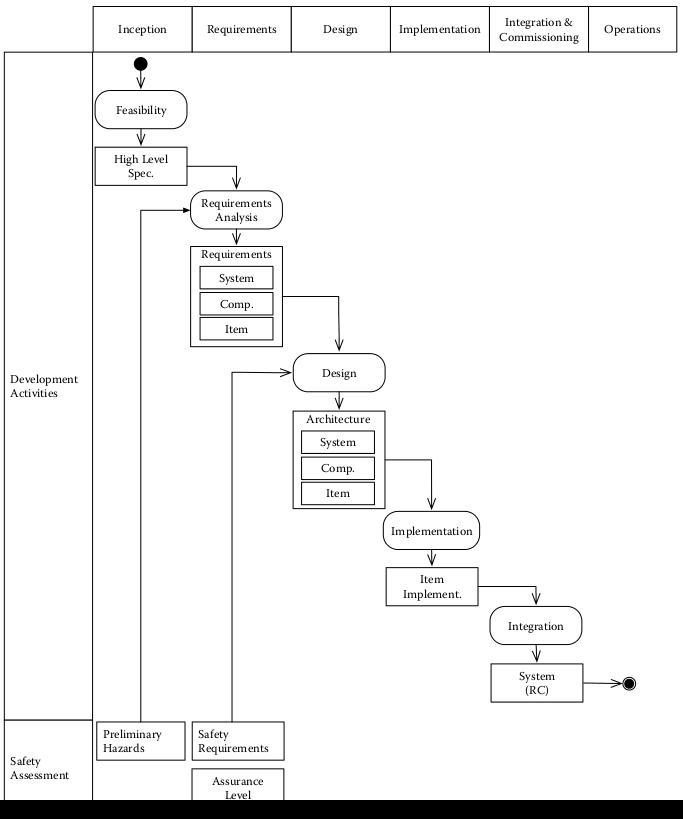
\includegraphics[width=\linewidth]{images/genDevFlow}
    \end{center}
\end{itemize}

\subsubsection*{Feasibility Study}
\begin{itemize}
    \item assess technical feasibility, first high-level definition of functions
    \item[\follows] feasibility document
    \item 5M model
    \begin{description}
        \item[Mission] main purpose of a system, success criteria, strategic objectives
        \item[Man] human factor, risk, constraints, training
        \item[Machine] the platform that will be used to achieve mission goal
        \item[Media] environment in which system will operate
        \item[Management] set of procedures, regulations necessary for operation, maintenance and disposal of system
    \end{description}
\end{itemize}

\subsubsection*{Requirement Analysis}
\begin{itemize}
    \item outputs of feasibility study are refined to produce sufficiently detailed and precise description
    \item[\follows] requirements document (or set thereof)
    \item often contractual agreement
    \item three tasks
    \begin{description}
        \item[Requirements elicitation] elicit system characteristics
        \item[Requirement specification] organize requirements, annotated with meta-information
        \item[Requirement validation] confirm, that requirements describe ``the right system''
    \end{description}
\end{itemize}

\subsubsection*{Design}
\begin{itemize}
    \item determine architecture of system \follows diagrams, documents, blueprints
    \item allocation of safety requirements has consequences:
    \begin{itemize}
        \item imposes specific design choices, e.g. adoption of TMR for critical components
        \item imposes constraints on development process that must be adopted
    \end{itemize}
\end{itemize}

\subsubsection*{Implementation and Integration}
\begin{itemize}
    \item build leaf elements of system during \emph{implementation}
    \item assemble and integrate components during \emph{integration}
\end{itemize}

\subsubsection*{Hierarchical Design of Systems}
\begin{itemize}
    \item time flows from top to bottom
    \item at first level of detail (system level) requirements are for the whole system
    \item at second level of detail (component level) architecture and requirements are decomposed, refined and allocated to components
    \item at third level (item level, items are assumed to be simple), refine components into requirements, basis for item implementation
    \begin{center}
        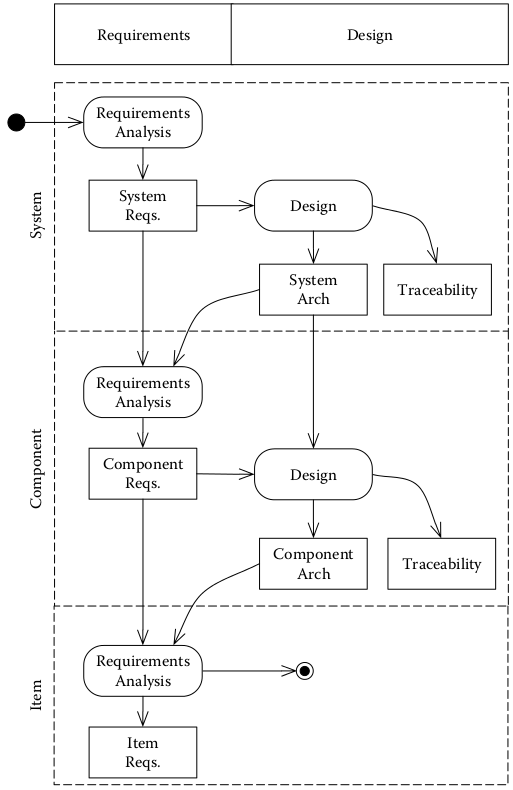
\includegraphics[width=\linewidth]{images/hierarchical.png}
    \end{center}
\end{itemize}

\subsection*{Testing Workflow}
\begin{itemize}
    \item testing activities span throughout system development, may continue in production
    \begin{description}
        \item[development testing] during development
        \item[verification testing] verification of final product
        \item[production testing] ensure every does not have fabrication defects
    \end{description}
    \item testing contains different stages
    \begin{description}
        \item[planning stage] scope, plan general objectives are drafted
        \item[definition phase] testing strategy is defined, test cases are constructed
        \item[execution phase] test campaign is conducted, results are reported
    \end{description}
\end{itemize}

\subsubsection*{Acceptance Test Definition}
\begin{itemize}
    \item verify system compliance with requirements
    \item testing performed in test cases
    \item tests according to development stage
    \begin{description}
        \item[Analysis] use of mathematical modeling and analytical techniques
        \item[Demonstration] providing means to demonstrate a requirement is satisfied
        \item[Inspection] visual examination of realized end product
        \item[Test] use end product to obtain detailed data needed to verify compliance with the requirements
    \end{description}
\end{itemize}

\subsubsection*{Integration Test Definition}
\begin{itemize}
    \item ensure, that subsystems interact as expected \follows test integration document
\end{itemize}

\subsubsection*{Unit Test Definition}
\begin{itemize}
    \item verify module or item
    \item typically look at actual implementation
\end{itemize}

\subsubsection*{Test Execution}
\begin{itemize}
    \item require delivery of implemented items, components and system:
    \begin{description}
        \item[Unit Test Execution] execute unit tests, often automated, code that breaks previous assumptions, fail the test
        \item[Integration Tests] execute integration tests
        \item[Acceptance Tests] ensure, that delivered system correctly implements the requirements
    \end{description}
    \item tests produce several version:
    \begin{description}
        \item[alpha release] early system releases
        \item[beta release] more mature system
        \item[RC-$N$] Release Candidate, number $N$
    \end{description}
    \item testing can not prove absence of faults
\end{itemize}

\subsection*{Safety Assessment Workflow}
\begin{itemize}
    \item two different phases, complementary goals
    \begin{itemize}
        \item during system development (requirements, design, implementation) \follows ``constructive'' role: guide design activities, ensure safety goal
        \item during integration \follows ``destructive role'', demonstrate whether system is safe, actually meets safety requirements \follows question all design hypotheses
    \end{itemize}
    \item techniques are the same (e.g. fault tress, FMECAs) but purpose is different
\end{itemize}

\subsubsection*{Preliminary Hazard Analysis (PHA) and Hazard Analysis (HA)}
\begin{itemize}
    \item goal: identify potential hazards and safety risks
    \begin{description}
        \item[PHA] when initial information is available
        \item[HA] when more detailed and more consolidated information is available
    \end{description}
    \item strategies to manage hazards
    \begin{enumerate}
        \item \emph{Design for minimum risk}: design to eliminate risks or reduce to acceptable level
        \item \emph{Incorporate safety devices}: if risks cannot be eliminated, reduce risk via use of fixed automatic or other safety design features, provisions for periodic functional checks
        \item \emph{Provide warning devices}: neither design nor safety devices can effectively eliminate identified risks or adequately reduce risk, produce adequate warning signal
        \item \emph{Develop procedures and training} where risk elimination is impractical through design selection or safety and warning devices \follows procedures and training
    \end{enumerate}
\end{itemize}

\subsubsection*{Determination of Assurance Levels}
\begin{itemize}
    \item components are not equally critical \follows rigor of development due to \emph{assurance levels}
    \item classify for effects of violation of safety requirements
    \begin{description}
        \item[Catastrophic] malfunction causes unsafe operational conditions
        \item[Hazardous] malfunction severely reduces operational safety, might cause severe stress on operators and have adverse effects on occupants
        \item[Major] malfunction significantly reduces safety margins and increases workload of operators, causing distress to occupants
        \item[Minor] if malfunction causes slight reduction in safety margins, slight increase in workload, some inconvenience for occupants
        \item[Negligible] malfunction has no effect on safety
    \end{description}
    \item probability is another factor
    \begin{center}
        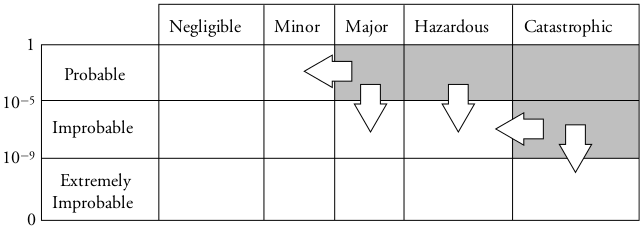
\includegraphics[width=\linewidth]{images/riskProb.png}
    \end{center}
    \item NASA assurance level
    \begin{enumerate}
        \item Determine \emph{risk index} of software component, probability and impact of failures
        \item Determine \emph{control category}, look at characteristics of software
        \item Determine \emph{software risk index}, number from $1$ to $5$, correspond to required safety effort necessary for its development
    \end{enumerate}
\end{itemize}

\subsubsection*{Preliminary Safety Assessment (PSA)}
\begin{itemize}
    \item perform safety analysis on system while its being developed
    \item interest  between preliminary safety assessment and design in the case of hierarchical development process
    \item outputs are requirements, architecture and list of hazards
    \item activities proceed to next level of refinement (component level) \follows specification of each component
\end{itemize}

\subsubsection*{Safety Assessment (SA)}
\begin{itemize}
    \item proceed in bottom-up fashion, from component to system level, verfiy the hypotheses made during design
    \item safety verification include
    \begin{description}
        \item[Item and Component Safety Assessment] lower levels of architecture are verified, Fault Tree Analysis, FME(C)A and Common Cause Analysis
        \item[System Safety Assessment] verify architecture, Fault Tree Analysis, FME(C)A and Common Cause Analysis
    \end{description}
\end{itemize}

\subsubsection*{Common Cause Analysis (CCA)}
\begin{itemize}
    \item in case of systematic failures \follows redundancy not useful
    \item three kinds of common cause analysis (SAE)
    \begin{description}
        \item[Common Mode Analysis] systematic errors in development process, usually done via checklists
        \item[Particular Risk Analysis] considers external events that invalidate the independence of components (e.g. fire, snow, lightning, ruptures, leakages, \dots)
        \begin{enumerate}
            \item Determine scope of analysis (the risk to analyze)
            \item Define the models regulating the risk
            \item Define the effects of the risk base on the model
            \item Determine the failures on the systems components (based on effects of risk)
            \item Determine how the failures propagate to the rest of the system
        \end{enumerate}
        \item[Zonal Safety Analysis] physical proximity can invalidate the independence of components
        \begin{description}
            \item[Identify system's zone] the different zones of the system are identified, for many systems such zones are predefined and standardized
            \begin{description}
                \item[list components] all components of zones
                \item[list hazards] all hazards pertaining to the zone are listed
                \item[perform analyses] identify effect of hazard (FMEA, FTA)
                \item[define mitigation rules] strategies how to deal with hazard due to zonal installation
            \end{description}
        \end{description}
    \end{description}
    \item redundancy based upon different designs
\end{itemize}

\subsubsection*{Common Cause Analysis and Software}
\begin{itemize}
    \item redundancy does not really improve with software
    \begin{itemize}
        \item failures in software primarily design problems
        \item no variations, all copies are identical, will fail in the same way
    \end{itemize}
    \item use \emph{diversity}, independent software versions by independent teams, different tools and programming languages \follows different teams may still produce coincident errors
\end{itemize}

\subsubsection*{Operating and Support Hazard Analysis (O\&SHA)}
\begin{itemize}
    \item identify, analyze and evaluate the possible hazard to people, environment and property associated to system life cycle
    \item outputs are changes to design, procedures, testing, training, \dots
\end{itemize}

\subsection*{Certification Management Workflow}
\begin{itemize}
    \item safety-critical systems may be certified in certain areas (EASA - European Aviation Safety Agency, NRC - Nuclear Regulatory Commission)
    \item product certification workflow helps ensure that certification proceeds as smoothly as possible, involve certification agency as soon as possible
    \item documents:
    \begin{description}
        \item[Contractual activities] ensure, that all legal aspects and agreements between certification authority and applicant are properly taken care of
        \item[Managerial activities] all activities related to managing the certification process, includes: planning, monitoring, ensuring a proper integration of technical certification activities in other workflows
        \item[Technical activities] activities related to evaluating compliance of system with target regulations and safety goals.
    \end{description}
    \item certification phases, transitions happen with audits/ checklists
    \begin{enumerate}
        \item conceptual design phase
        \begin{itemize}
            \item \emph{ensure early , value added, joint involvement with an expectation to surface critical areas and the related regulatory issues}
            \begin{description}
                \item[process orientation]  partnership between applicant and certification authority is established \follows ``Partnership for Safety Plan'' (PSP)
                \item[pre-project guidance, familiarization briefings] discussion about policies, regulations, product characteristics \follows identify potential issues, risks, points of attention
                \item[certification planning] outlines certification plan, includes data to be submitted, methods of compliance, schedule
            \end{description}
        \end{itemize}
        \item requirement definition phase
        \begin{itemize}
            \item ensure that certification project is up and running
            \begin{description}
                \item[project setup] set up organizational structure, team, tools
                \item[issues book] repository of \emph{issue papers}, which describe technical and regulatory issues
                \item[certification basis] how compliance with safety regulations will be shown
            \end{description}
        \end{itemize}
        \item compliance planning phase
        \begin{itemize}
            \item define activities for actual implementation of certification
            \item participation of certification authority needed on every decision on critical stuff
        \end{itemize}
        \item implementation phase
        \begin{itemize}
            \item actual implementation of certification takes place
            \item \emph{conformity inspection}: provide documentation of compliance with design,
            \item tests, inspections, analyses
        \end{itemize}
        \item post-certification phase
        \begin{itemize}
            \item define stuff for managing and maintaining certification through life-cycle
        \end{itemize}
    \end{enumerate}
    \item \emph{issues book} properly trace and deal with issues\\
    compliance can be shown by
    \begin{description}
        \item[standard techniques]  issue is shown to be properly handled via safety analysis technique
        \item[equivalent level of safety] compensating factors are put in place
        \item[special condition] adoption of unusual design feature or technique does not allow standard practices
    \end{description}
\end{itemize}

\subsection*{Project Management Workflow}
\begin{shaded}
    ``The application of knowledge, skills, tools and techniques to project activities to meet project requirements.''
\end{shaded}
\begin{itemize}
    \item \emph{PRoject IN a Controlled Environment} (PRINCE2) (British)
    \item \emph{Project Management BOdy of Knowledge} (PMBOK) (American)
    \begin{center}
    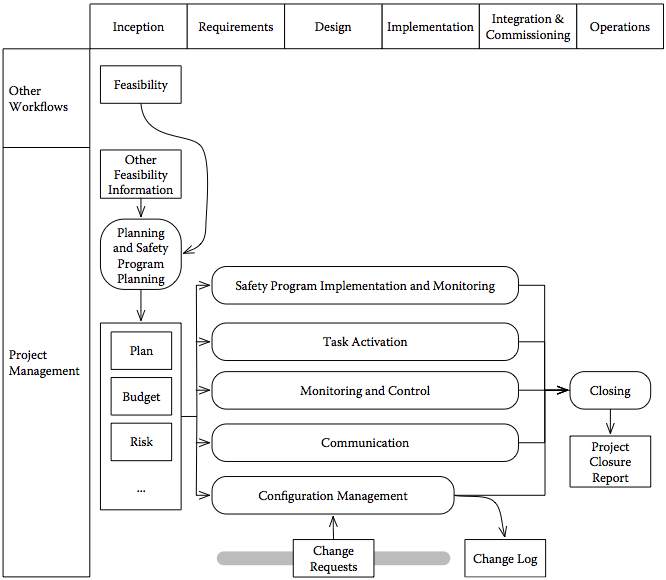
\includegraphics[width=\linewidth]{images/management.png}
    \end{center}
\end{itemize}

\subsubsection*{Safety Process Definition and Tailoring}
\begin{itemize}
    \item customize development process, adapt it to level of formality required
    \item output is a document that describes (minimum):
    \begin{itemize}
        \item how safety program will be implemented, techniques and standards
        \item resources responsible for implementation of safety plan (\follows dedicated safety team)
        \item how safety program and safety team fit into overall project structure, lines of communication
    \end{itemize}
\end{itemize}

\subsubsection*{Safety Program Implementation and Monitoring}
\begin{itemize}
    \item ensure that safety program is implemented according to standards and rules defined for project
    \item safety manager responsible for
    \begin{itemize}
        \item maintain log of identified hazards and residual hazards
        \item formally approving any residual hazard
        \item communicate hazards and residual hazards to end user
    \end{itemize}
\end{itemize}

\subsubsection*{Other Management Activities}
\begin{description}
    \item[planning] forecasting the dimensions of project
    \item[task activation] project manager activates and verifies termination of tasks according to plan
    \item[monitoring and control] data about progress is collected and compared with baseline plans
    \item[communication] project manager is responsible for information flow
    \item[configuration management] provide visibility and control over changes
    \item[closing] asses project after end
\end{description}

\subsection*{Tool Support}
\begin{center}
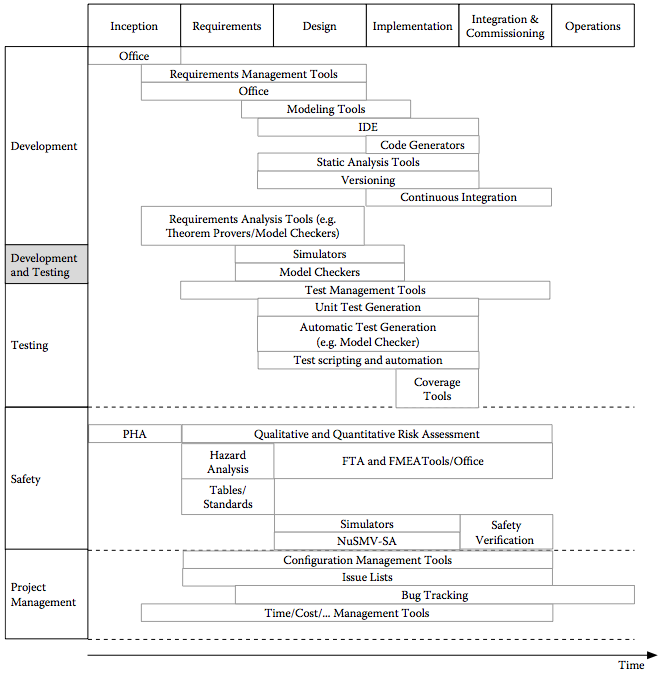
\includegraphics[width=\linewidth]{images/toolSupport.png}
\end{center}

\subsubsection*{Supporting the Development Workflow}
\begin{description}
    \item[requirement management tools]
    \begin{itemize}
        \item annotate enrich requirements with meta-information
        \item maintain traceability
    \end{itemize}
    \item[requirement analysis tool] reason about requirements, provide information about consistency/ completeness, often with formal representations
    \item[modeling tools, simulators, code generators] blur distinction between design, development and testing
    \begin{itemize}
        \item simulation: SPICE, MATLAB Simulink
        \item formal verification: SPIN; NuSMV, theorem provers
    \end{itemize}
    \item[static analysis tools] IDEs, certified compilers
    \item[versioning systems] coherent management of whole sets of files
    \item[build and continuous integration] simplify management of complex software systems
    \item[configuration management]
    \item[issue and bug-tracking management]
\end{description}

\subsubsection*{Supporting the Testing Workflow}
\begin{itemize}
    \item tools, that help maintain specification of tests, often web based, trace test results, integration with bug-tracking tools
    \item tools to support automatic generation and execution of tests, based on model checkers and static analysis, automatic generation of test cases
    \item tools to support evaluation of tests, verify completeness of tests, code coverage
\end{itemize}

\subsubsection*{Supporting the Safety Analysis Workflow}
\begin{itemize}
    \item tools for management of safety-related information, FaulTree+, semantically meaningful way of drawing and managing fault trees
    \item tools for quantitative assessment of risks and hazards, based on probability theory, monte carlo simulation, markov analysis
    \item tools for qualitative assessment of risks and hazards, tools like NuSMV-SA, automatic generation of fault trees (?)
\end{itemize}

\end{document}
